\documentclass[fleqn,10pt]{wlscirep}
\usepackage[utf8]{inputenc}
\usepackage[T1]{fontenc}
\usepackage{eucal}
\usepackage[mathcal]{eucal}

\usepackage{bm}
\newcommand{\ydnote}[1]{\textcolor{red}{#1}}
\title{  Fault detection and Diagnosis System for CSTR reactor with a hybrid knowledge-machine learning approach}

\author[1,*]{Yong Dou(yd2373)}

\affil[1]{Columbia University, Department of Chemical Engineering ,New York, NY}

\affil[*]{e-mail:yd2373@columbia.edu}


\begin{abstract}

\end{abstract}
\begin{document}

\flushbottom
\maketitle

\thispagestyle{empty}

\noindent \textbf{Key points:} Neural Network, Knowledge based system, CSTR, Fault detection}


\section*{Article types in Nature Reviews Physics}
\subsection*{Introduction}
nonisothermal \cite{bruns1977nonlinear}




\subsection*{Perspective}
There are some hidden paramereeris that are still very important 

\subsection*{CSTR system and heat transfer}

constant density and isothermal condition. The advange including good temperature/ system, mulyiphase,  control, low and easy operating cost and continous operatation with some disadvange of low conversion rate and \ydnote{poor poor agitation}  

we assume this is a first order exothermic reaction and in a well mixed (no spatial difference for the reactions) steady state the very basic equations are 

\begin{equation}
    Fi_{in}-Fi_{out}+V ri
\end{equation}
\begin{equation}
    X=\frac{Fi_{in}-Fi_{out}}{Fi_{in}}
\end{equation}
\begin{equation}
    X=\frac{Fi_{in}-Fi_{out}}{Fi_{in}}
\end{equation}
\begin{equation}
      V=\frac{Fi_{in} X}{-rA}
\end{equation}

\ydnote{ Levenspiel Plot}
   
\begin{equation}
    q(C_{inlet}-C_{reaction})=C_A Vk(T_{reactor})
\end{equation}
\begin{equation} 
    q \rho \mathcal{C}(T_{inlet}-T_{reactor})+V(-\Delta H)k(T_{reactor}) C_{reactor}=(T_{outlet}-T_{inlet})Q_{cool} \mathcal{C}
\end{equation}
\begin{equation} 
    k(T_reactor)=k(T_{inlet})Exp\left[\frac{E}{RT_{inlet}} \frac{T{reactor}-T_{inlet}}{T{reactor}}\left]
\end{equation}
There have been lots of report on the analytical or numerical analysis of the above differential equation with or witout time \cite{balakotaiah1981analysis}  dynamics bahavors\cite{schmidt1981dynamic}, nontermal \cite{hamer1981dynamic} experiment\cite{teymour1989dynamic,teymour1992dynamic} ,\cite{teymour1992dynamic2}
complex reaction \cite{scott1983reversible,lin1981multiplicity}

q is the hidden parameter





\subsection*{fault diagnose in CSTR }
the ann\cite{hoskins1991fault} with physical explanation
taxonoy with signs\cite{chang1990line}

knowledge based system with a hierarchical Taxonomy  \cite{terpstra1992real}
internal fault(DON'T HAVE CHILDREN) and external fault(HAVE CHILDREN ), and unknown fault. pump valve pipe(feed and coolant), CSTR TRANPOSRT , MIXER VESSEL AND 
hybrid NERUAL NETWORK is also used in detecting the \cite{ozyurt1996hybrid}
these papers are  limited to the tools and 
fuzzy nertail network\cite{zhang1996process} much slower at that time

BY PCA, some physics meaning will be dropped 

there are step
\begin{itemize}
    \item learn the existenc of faulte
    \item isoltae the type of fault
    \item learn the physical cause
\end{itemize}

\ydnote{the output recommedication }

\bibliography{sample}

\noindent \textbf{For Reviews only, highlighted references (optional)} Please select 5–-10 key references and provide a single sentence for each, highlighting the significance of the work.

\section*{Acknowledgements (optional)}
The authors thank Erwin the Cat for useful discussions. Please edit as necessary.

\section*{Author contributions}
The authors contributed equally to all aspects of the article. Please edit as necessary. Note that the information must be the same as in our manuscript tracking system.

\section*{Competing interests}
The authors declare no competing interests. Please edit as necessary. Note that the information must be the same as in our manuscript tracking system.

\section*{Publisher’s note}
Springer Nature remains neutral with regard to jurisdictional claims in published maps and institutional affiliations.

\section*{Supplementary information (optional)}
If your article requires supplementary information, please include these files for peer-review. Please note that supplementary information will not be edited.

\newpage
\section*{Box 1 (Optional)}
This is a Box, which can contain a figure, and which should have no more than 300 words of text.

\begin{figure}[ht]
\centering
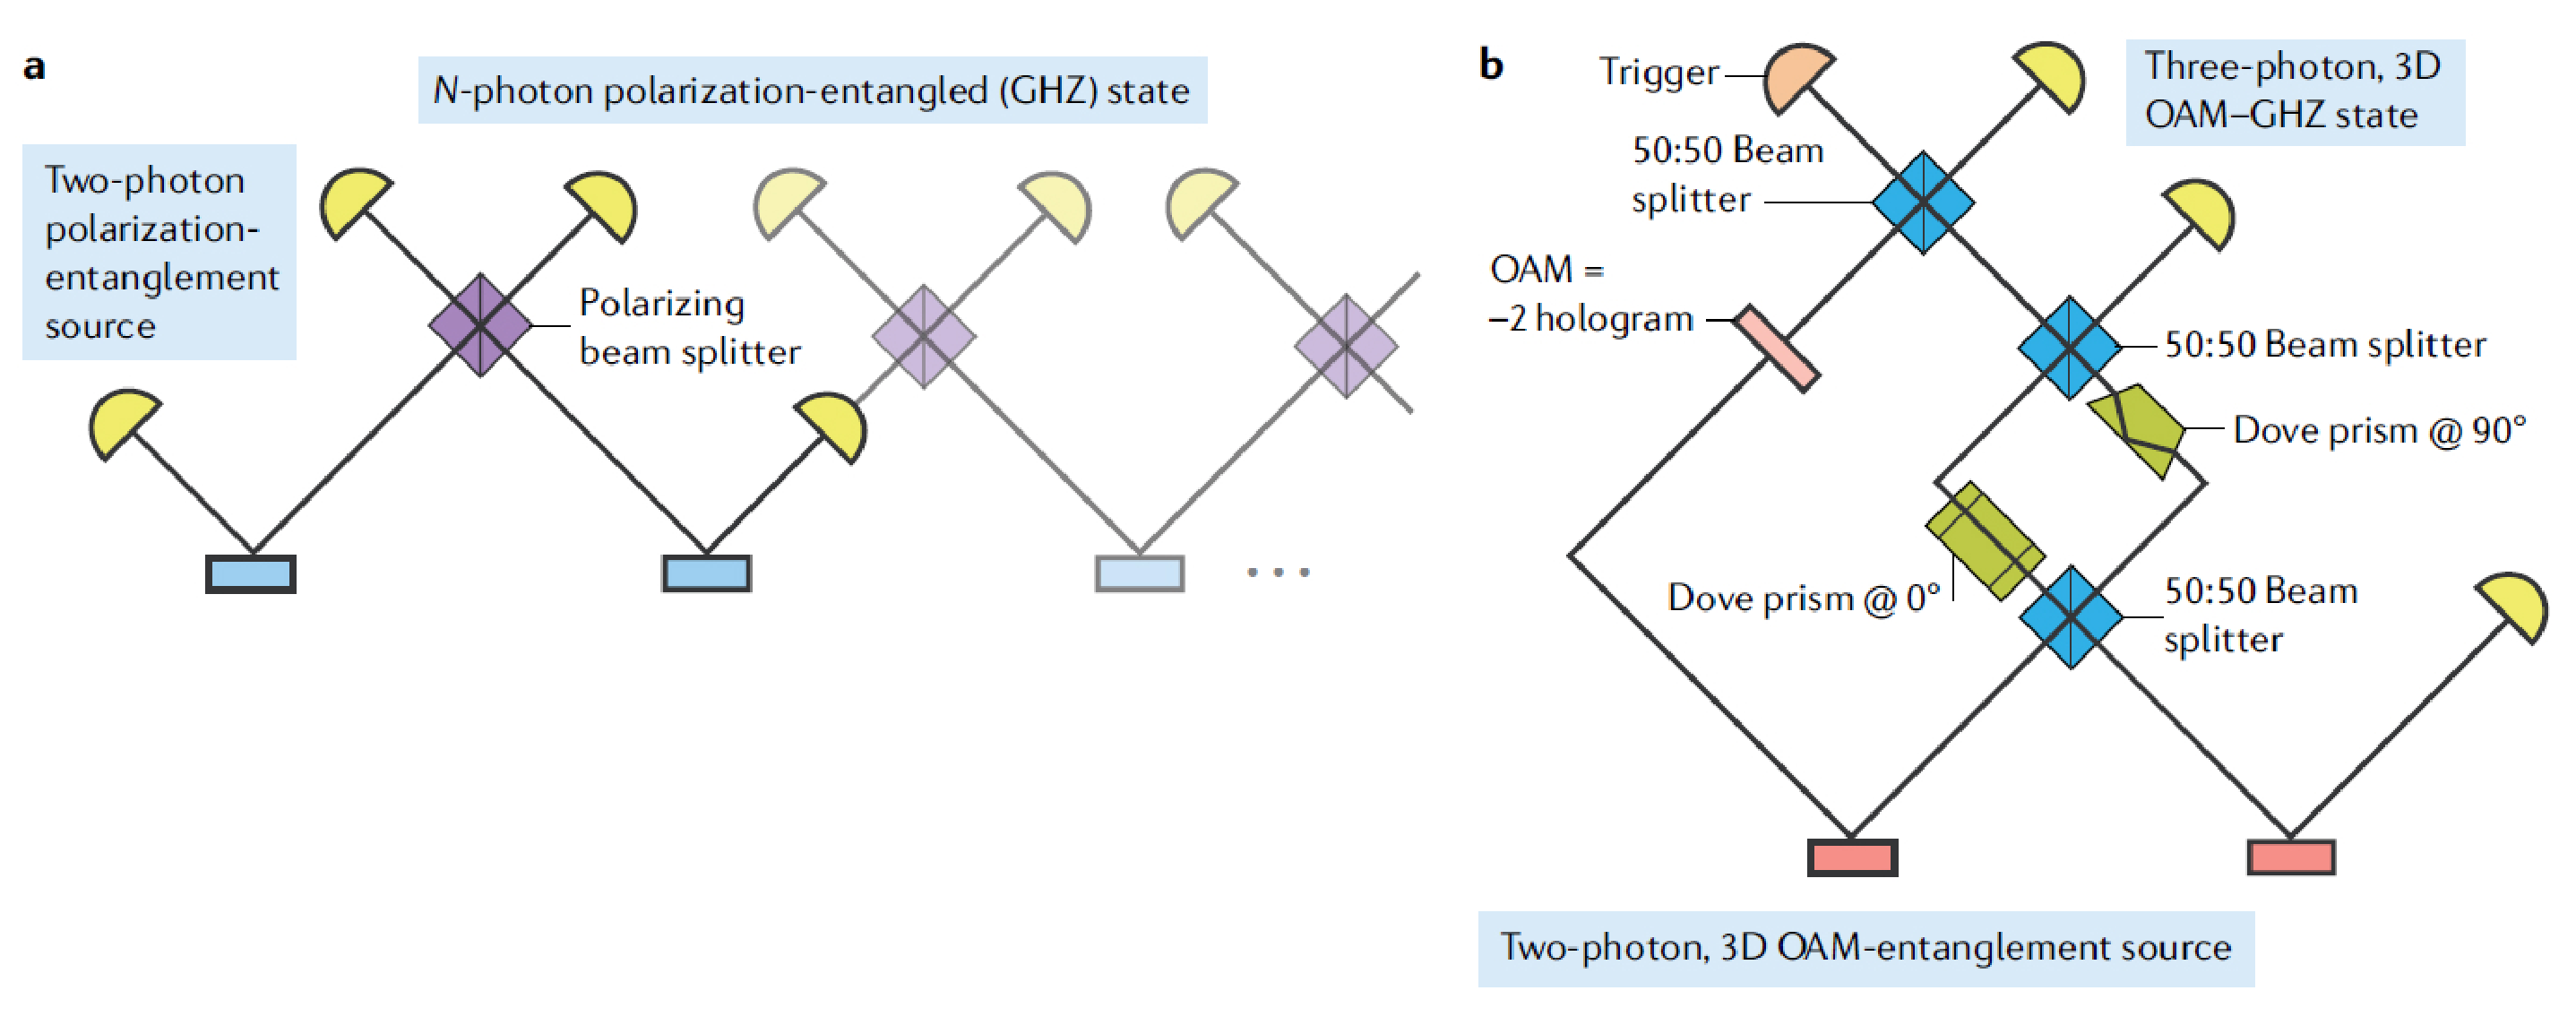
\includegraphics[width=\linewidth]{fig}
\caption{The figure caption should start with a title explaining the figure. Figures should be self-consistent so please redefine all acronyms and define all symbols. Example: GHZ, Greenberger–Horne–Zeilinger, OAM, orbital angular momentum. Please provide credit lines for panels reproduced from the literature. Example: Panels a and b are reproduced from Ref. \cite{TR}.}
\label{fig}
\end{figure}

\begin{table}[ht]
\centering
\begin{tabular}{|l|l|l|}
\hline
Particle & Mass & Charge \\
\hline
Electron & $9.10938356(11)\times10^{-31}$ kg & $-1e$ \\
\hline
Proton & $1.672621898(21)\times10^{-27}$ kg & $+1e$ \\
\hline
Neutron & $1.674927471(21)\times10^{-27}$ kg & $0$ \\
\hline
\end{tabular}
\caption{\label{tab}Tables have titles but no captions are allowed. However, all symbols and acronyms used in a table should be defined in a footnote. Example: Here $e$ is the elementary charge.}
\end{table}

\section*{Glossary terms (optional)}
It is possible  to include glossary terms to define some technical terms. For each glossary term, please provide a short (maximum 30 word) definition. Please list these in order of first appearance in the text. In the published version, they will appear in the margins of the document. 

Example: \\
\textbf{Lam\'e parameters:} A possible pair of parameters that characterize the Cauchy elasticity tensor in an isotropic homogeneous medium. The second Lam\'e parameter is identical to the shear modulus.



\end{document}